\documentclass[a4paper, 9pt, landscape]{article}
\usepackage[scaled=0.92]{helvet}
\usepackage{multicol}
\usepackage{calc}
\usepackage{ifthen}
\usepackage[landscape]{geometry}
%\usepackage{hyperref}

\usepackage{newtxtext} 

%for strikeout
\usepackage{ulem}

%For editing parbox
\usepackage[table]{xcolor}
%For editing itemise margins, reduce iterm separaion and list separation
\usepackage{enumitem}
% For math
\usepackage{amsmath,amsthm,amsfonts,amssymb}

%For pictures / figures
\usepackage{color,graphicx,overpic}
\graphicspath{ {./images/} }


\pdfinfo{
  /Title (CS4226.pdf)
  /Creator (Ger Teck)
  /Author (Ger Teck)
  /Subject ()
  /Keywords (tex)}

%% Margins for PAPER

%% Margins for A4 PAPER
\geometry{top=0.5cm,left=0.5cm,right=0.5cm,bottom=0.5cm}
\pagestyle{empty}
\newenvironment{tightcenter}{%
  \setlength\topsep{0pt}
  \setlength\parskip{0pt}
  \begin{center}
}{%
  \end{center}
}

% Redefine section commands to use less space
\makeatletter
\renewcommand{\title}{\@startsection{section}{1}{0mm}%
                                {-1ex plus -.5ex minus -.2ex}%
                                {0.5ex plus .2ex}%x
                                {\normalfont\large\bfseries}}
\renewcommand{\section}{\@startsection{subsection}{2}{0mm}%
                                {-1explus -.5ex minus -.2ex}%
                                {0.5ex plus .2ex}%
                                {\normalfont\normalsize\bfseries}}
\renewcommand{\subsection}{\@startsection{subsubsection}{3}{0mm}%
                                {-1ex plus -.5ex minus -.2ex}%
                                {1ex plus .2ex}%
                                {\normalfont\small\bfseries}}

\makeatother

% Define BibTeX command
\def\BibTeX{{\rm B\kern-.05em{\sc i\kern-.025em b}\kern-.08em
    T\kern-.1667em\lower.7ex\hbox{E}\kern-.125emX}}

\setcounter{secnumdepth}{0}
\setlength{\parindent}{0pt}
\setlength{\parskip}{0pt plus 0.5ex}

%% this changes all items (enumerate and itemize, reduce margins)
\setlength{\leftmargini}{0.5cm}
\setlength{\leftmarginii}{0.5cm}
\setlist[itemize,1]{leftmargin=2mm,labelindent=1mm,labelsep=1mm, itemsep = 0mm, before=\justifying}
\setlist[itemize,2]{leftmargin=2mm,labelindent=0.5mm,labelsep=0.5mm, itemsep = -0.2mm, topsep=-0.2mm, before=\justifying}
%\setlist{nosep}

\usepackage[document]{ragged2e}

% -------------------------------------------------------------------------------

% START OF DOCUMENT HERE

\begin{document}
\raggedright
\footnotesize
\begin{multicols*}{3}

% multicol parameters
% These lengths are set only within the two main columns
\setlength{\columnseprule}{0pt}
\setlength{\premulticols}{1pt}
\setlength{\postmulticols}{1pt}
\setlength{\multicolsep}{2pt}
\setlength{\columnsep}{2pt}

\title{CS4226 Internet Architecture}
\centerline{AY25/26 Sem 1. github.com/gerteck}

\section{0. \underline{Introduction}}
\begin{itemize}
\item Internet Architecture Prerequisites: Basic network terms including host, packet, protocol, throughput, bottleneck link, store-and-forward, and autonomous systems.
\item Logical (five layers) and physical architecture (network of ASes). Pros and cons of packet switching versus circuit switching. Different components of end-to-end delay and relation to bandwidth, packet size, distance, propagation speed and queue size.
\item \textbf{CS3103}: Computer Networks Practice. Focus on practical, protocol level understanding (vertical view of protocol stack), with layers covered including data link, network and transport.
\item \textbf{CS4226}: Internet Architecture. Focus on theoretical, architectural and systemic (horiziontal ecosystem view). Cross layer architectural design, such as peer-to-peer networks
\end{itemize}	




\section{1. \underline{Performance Metrics}}

\subsection{Link Rate / Bandwidth / Capacity}
\begin{itemize}
    \item How many bits can be ``pushed'' onto a link per unit time. (Bandwidth)
    \item E.g. Cable: in Mbps, Fiber optics: $1 \sim 10$ Gbps, Ethernet: $3$ Mbps to $100$ Gbps
    \item Link rate related to transmission delay, or ``putting furniture into the moving van''.
\end{itemize}

\subsection{Throughput}
\begin{itemize}
    \item Throughput of a TCP/UDP flow. (End-to-End, includes propagation delay).
    \item How many bits are communicated / pushed throughout entire routing path per unit time.
\end{itemize}

\subsection{End-to-End Delay}
\begin{itemize}
    \item \textbf{Components}: Processing delay + Queueing delay + Transmission delay + Propagation delay
	 \item Processing (time taken by router/devices to process packet header), Queueing (time packet waits in buffer before it is transmitted, due to congestion), propagation delay (time taken for bit to travel from one end of link to the other.). Transmission delay is the time it takes for physical layer at source to send all bits of packet onto transmission medium.
	 \item \textbf{Variables}: Bandwidth, packet size, distance, propagation speed, queue size.
    \item Example: A packet of $L$ bits sent over a link with rate $R$ bits/sec takes. 
\end{itemize}

\subsection{Packet Switching: Store-and-Forward}
\begin{itemize}
    \item A packet of $L$ bits sent on a link with rate $R$ bps takes:
    \[
        \text{Transmission delay} = \frac{L}{R} \quad \text{seconds to push out.}
    \]
    
    \item \textbf{Store-and-forward}: entire packet must be at router before transmit to next link.
    \item E.g. $L = 7.5$ Mbits, $R = 1.5$ Mbps: Transmission delay per link = $\frac{L}{R} = 5$ sec. For 3 links: total delay $= \frac{3L}{R} = 15$ sec
\end{itemize}

\subsection{Other Metrics}
\begin{itemize}
\item \textbf{Reponse Time}: Time taken from request to response, aka \textit{round-trip time}, including server processing time etc. Traffic there and back may take different routing paths. Roughly 2x of end-to-end delay, but not exactly.
\item \textbf{Dropping Probability}, \textbf{Utilization}
\end{itemize}

\subsection{Packet Switching: Statistical Multiplexing}
\begin{itemize}
    \item Bandwidth shared on demand, no fixed pattern of packets. This is the origin of \textbf{queuing delay}. (Input rate $>$ output rate).
    \item Statistical multiplexing $\rightarrow$ efficient use of link capacity. Packet switching is more efficient to share resources among users. (Statistical: arrival of packets non-deterministic)
    \item Contrast with TDM (Time Division Multiplexing):
    \begin{itemize}
        \item TDM: each host gets same slot in a revolving frame.
        \item Statistical multiplexing: bandwidth allocated dynamically as needed.
    \end{itemize}
\end{itemize}

\subsection{Packet vs Circuit Switching}
\begin{itemize}
    \item Example: For Link capacity of 1 Mbps, where each user requires 100 kbps when active, active 10\% of time.
    \begin{itemize}
	    \item \textbf{Circuit switching} $\Rightarrow$ supports 10 users
		 \item \textbf{Packet switching} $\Rightarrow$ with 35 users, probability $>10$ active simultaneously is $<0.0004$.
	 \end{itemize}
    \item \textbf{Pros of packet switching}: Great for bursty, asynchronous data, Resource sharing, No call setup required.
    \item \textbf{Cons of packet switching}: Excessive congestion $\rightarrow$ packet delay and loss, requiring protocols for reliability and congestion control.
\end{itemize}


\subsection{Single-Server Queueing Model (Abstract System)}
\begin{itemize}
    \item Model (to understand queueing delay): one server with infinite queue.
    \item Arrival rate: $\lambda$ (packets per second).
    \item Service rate: depends on server capacity (e.g., 1.5 Mbps).
    \item Average queue length and waiting time linked by Little’s Law.
\end{itemize}
\centerline{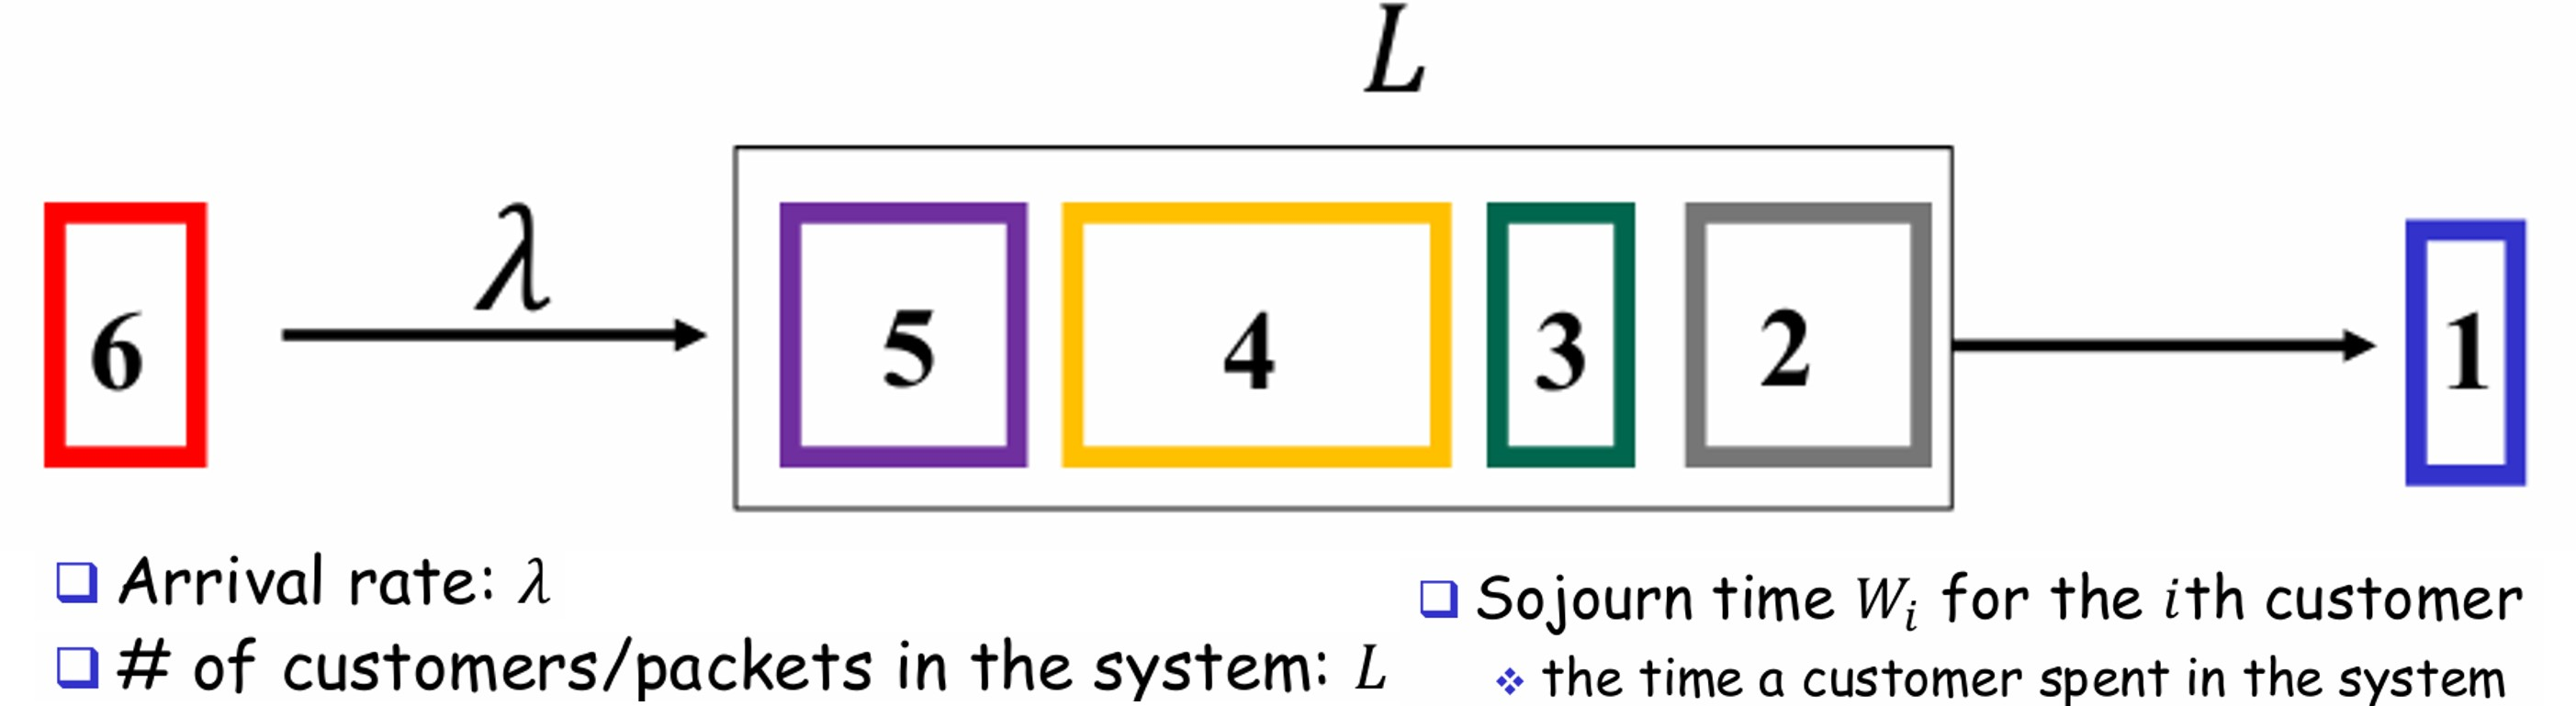
\includegraphics[width=0.6\linewidth]{littlesLaw}}

\subsection{Little’s Law}
\[
    L = \lambda W
\]
\begin{itemize}
    \item $L$: average number of customers in system
    \item $\lambda$: average arrival rate
    \item $W$: average sojourn time (time spent in system)
\end{itemize}
\textbf{Examples:}
\begin{itemize}
    \item SoC admits 1500 students per year, has 6000 students enrolled at any time. 
    \[
        W = \frac{L}{\lambda} = \frac{6000}{1500} = 4 \text{ years}
    \]
    \item If average queue length $=5$ packets and arrival rate $=100$/sec, then
    \[
        W = \frac{L}{\lambda} = \frac{5}{100} = 0.05 \text{ sec}
    \]
\end{itemize}


\section{2. \underline{Network Queueing Models}}


\subsection{Packet Flow: Arrival Pattern}
\begin{itemize}
    \item Arrival times: $t_i$; \quad Inter-arrival times: $T_i \equiv t_{i+1} - t_i$
    \item Model $T_i$s as independent, identically distributed (i.i.d.) random variable (r.v.) $T$
\end{itemize}
\centerline{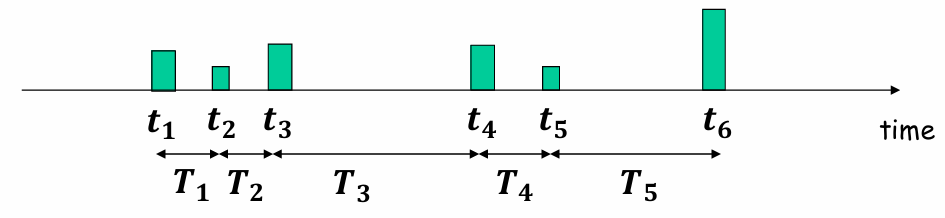
\includegraphics[width=0.6\linewidth]{packetArrivalModel}}

\subsection{Probability Basics and Recap}
\begin{itemize}
    \item Random experiment: outcome cannot be determined in advance
    \item Sample space $S$: set of all outcomes; \quad Event $E \subseteq S$: occurs if $s \in E$
    \item Probability function $P(E):  \quad 0 \le P(E) \le 1, \quad P(S) = 1 $
\end{itemize}

\subsection{Random Variables (r.v.)}
\begin{itemize}
    \item Random variable $X$ is a \textbf{mapping}: maps each outcome $s \in S$ to real value
    \item Distribution function $F(x) = P(X \le x)$
    \item Continuous r.v.: exists pdf $f(x) = \frac{d}{dx}F(x)$
    \item Independence: $f_{X,Y}(x,y) = f_X(x) f_Y(y)$
    \item Expectation:
    \[
        E[X] = \int_{-\infty}^\infty x f(x) dx \quad \text{or} \quad E[X] = \sum_x x P(X=x)
    \]
\end{itemize}

\subsection{Exponential Distribution (Time between Intervals)}
\begin{itemize}
    \item $T \sim \text{Exp}(\lambda)$ with $\lambda > 0$: (note interarrival times cannot be negative).
    \[
        f(x) =
        \begin{cases}
            \lambda e^{-\lambda x}, & x \ge 0 \\
            0, & x < 0
        \end{cases}
    \]
    
    \item \textbf{CDF $F(X)$: probability that event occurs within time x}, $P(T \le x)$
    \item $F(x) = P(T \le x) = \int_{0}^{x} \lambda e^{-\lambda u}\,du =  1 - e^{-\lambda x}, \quad x \ge 0$
    \item \textbf{Memoryless}: $P(T > s+t \mid T > s) = P(T > t)$
    \item \textbf{Expectation: (E[T]: Time till next event)}
    \[
        E[T] = \int_{0}^{\infty} x \, \lambda e^{-\lambda x} \, dx
    \]
    Integration by parts:
    \[
        E[T] = \left[ -x e^{-\lambda x} \right]_{0}^{\infty} +
        \int_{0}^{\infty} e^{-\lambda x} \, dx
        = 0 + \frac{1}{\lambda} \Rightarrow \; E[T] = \frac{1}{\lambda}
    \]
    \item \textbf{Physical meaning of $\lambda$:} 
    \begin{itemize}
        \item $\lambda$ is the \emph{arrival rate} (arrivals per unit time), unit: $\text{time}^{-1}$ (e.g., per second).
        \item On average, $\lambda$ events occur per unit time, or the mean interarrival time is $1/\lambda$.
    \end{itemize}
\end{itemize}

\subsection{\underline{Modeling Packet Flow}}


\subsection{Packet Arrival / Inter-arrival Times (Poisson Process, T$\sim$Exp($\lambda$).)}
\begin{itemize}
    \item Inter-arrival times $T_i \sim \text{Exp}(\lambda)$, i.e. each inter-arrival time is an RV with rate $\lambda$.
    \item \textbf{Arrival pattern}: Poisson process (\# arrivals in an interval follow Poisn. distribn.)
    \item \textbf{Properties}: Memoryless $\Rightarrow$ starting time irrelevant, and \\
    Merging: Poisson($\lambda_1$) (combination) Poisson($\lambda_2$) $\Rightarrow$ Poisson($\lambda_1 + \lambda_2$)
\end{itemize}

\subsection{Service Time (Exponential / i.i.d.)}
\begin{itemize}
    \item Service time (processing time) of packet $i$: $S_i$, under fixed link rate.
    \item $S_i$ are i.i.d. with mean $E[S] = 1/\mu$.
    \item \textbf{Physical meaning of $\mu$}: \emph{service rate}, avg packets per unit time that can be handled
    \item Depends on link rate and packet size, as packet size may vary, hence, take average.
\end{itemize}

\subsection{\underline{M/M/1 Model} {\tiny M (Markovian Poisson arrival process), M (Markovian memoryless service time), 1 (\# servers)  }}

\centerline{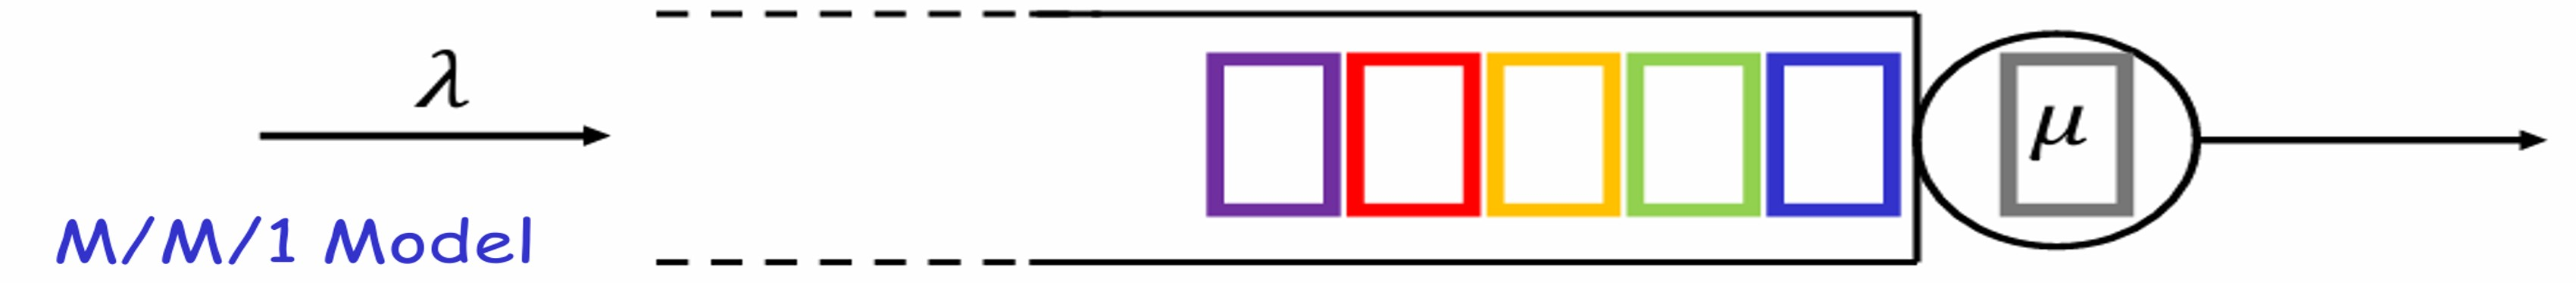
\includegraphics[width=0.8\linewidth]{mm1Model}}
\begin{itemize}
    \item Assumptions:
    \begin{itemize}
        \item Single server, infinite queue size, 
        \item Poisson \underline{arrivals rate $\lambda$}, Exponential \underline{service time rate $\mu$}
        \item Independent arrivals and service, FIFO service discipline
    \end{itemize}
    \item \textbf{Utilization $\rho$}| (\% time or probability of observation that server busy):
    \[
        \rho = \frac{\lambda}{\mu}, \quad \text{need } \lambda < \mu \text{ for stability}
    \]
\end{itemize}


\subsection{Birth-Death Process}
\centerline{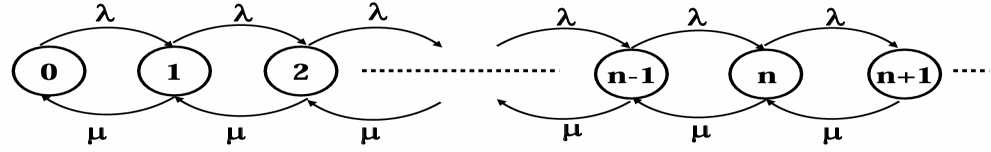
\includegraphics[width=0.8\linewidth]{birthDeath}}
\begin{itemize}
    \item State Transition Diagram for M/M/1 System.
    \item System state $L(t)$ = (random) number of users in system.
    \item Transitions: $ i \to i+1 \text{ at rate } \lambda, \quad i \to i-1 \text{ at rate } \mu $
\end{itemize}

\subsection{Stationary Distribution (Long-term behavior of System)}
\begin{itemize}
    \item For a M/M/1 system, denote $\pi_i$ as \% time exactly $i$ packets in system (ie. server + queue) / probability $P=\{L=i\}$ of random observation of $i$ packets in system.
    \item $\pi_i= P(L=i) = (1-\rho) \rho^i$,  (follows a geometric distribution)
    \item $\pi_0 = 1-\rho$ (utilization), and $\sum_i \pi_i = 1$
\end{itemize}

\subsection{M/M/1 Results}
\begin{itemize}
    \item Avg. \# packets in system: $ E[L] = \frac{\rho}{1-\rho} $
    \item Avg. sojourn time (system delay): $ E[W] = \frac{1}{\mu - \lambda} $
    \item Avg. \# packets in queue: $ E[Q] = \frac{\rho^2}{1-\rho} $
    \item Avg. queueing delay of packets: $E[D] = E[W] - \frac{1}{\mu} $
	\item If $\lambda \ge \mu$, server keep up w. arrivals and queue grows without bound.  
	      In particular, $\lambda = \mu$ is unstable (graphically approaches vertical asymptote at $\lambda = \mu$):
	      \[
	        E[L] = \frac{\rho}{1-\rho} \to \infty, \quad
	        E[W] = \frac{1}{\mu - \lambda} \to \infty
	      \]
	      Stability requires $\lambda < \mu$ (i.e., $\rho < 1$). ($\lambda = \mu$ insufficient bc. randomness).
\end{itemize}

%% LECTURE 2 STOPPED HERE & ----------------------------------------------------------------------

\subsection{\underline{Heavy Notation (Queueing Systems)}}
\centerline{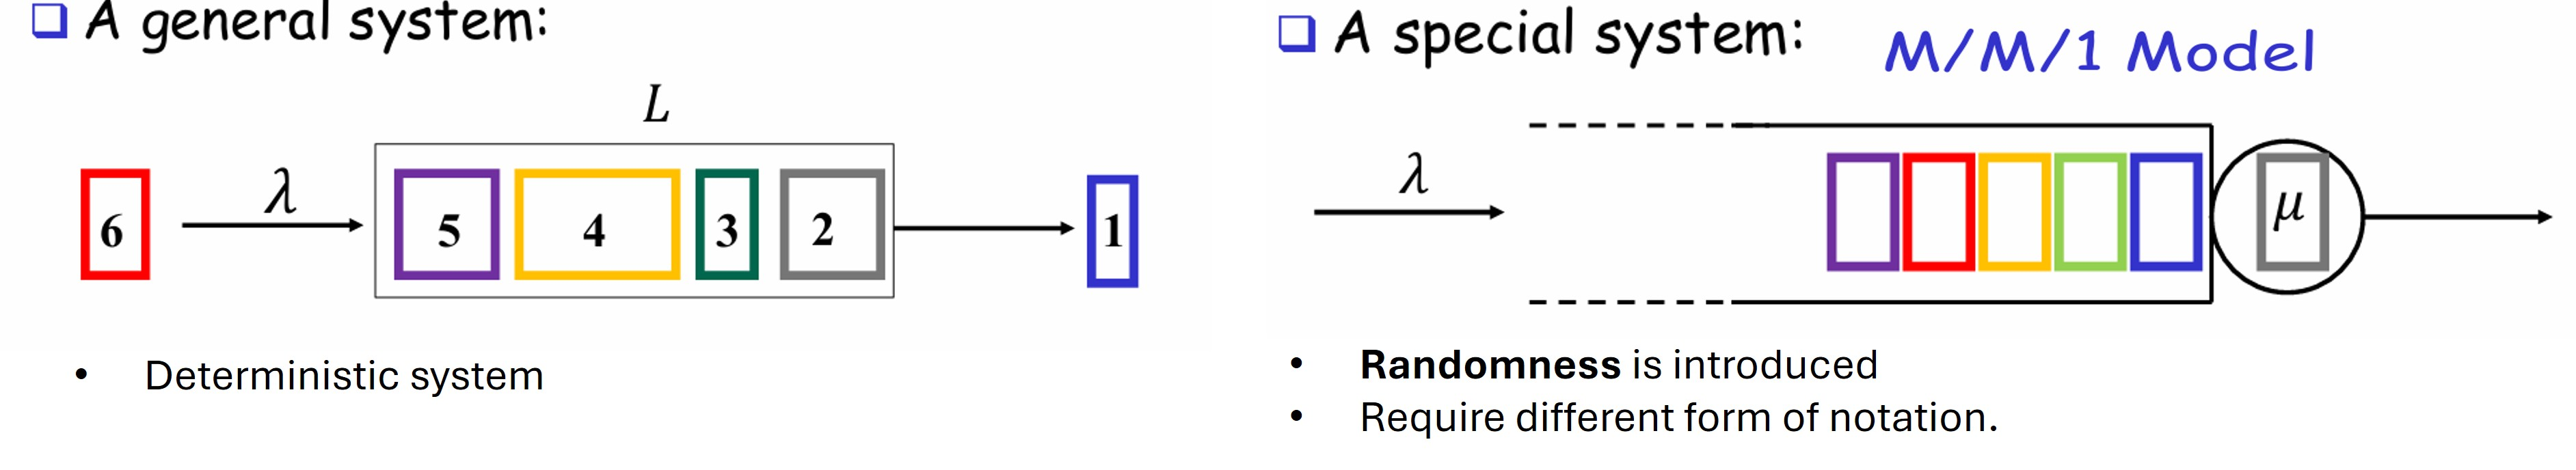
\includegraphics[width=1\linewidth]{models}}
\null
\centerline{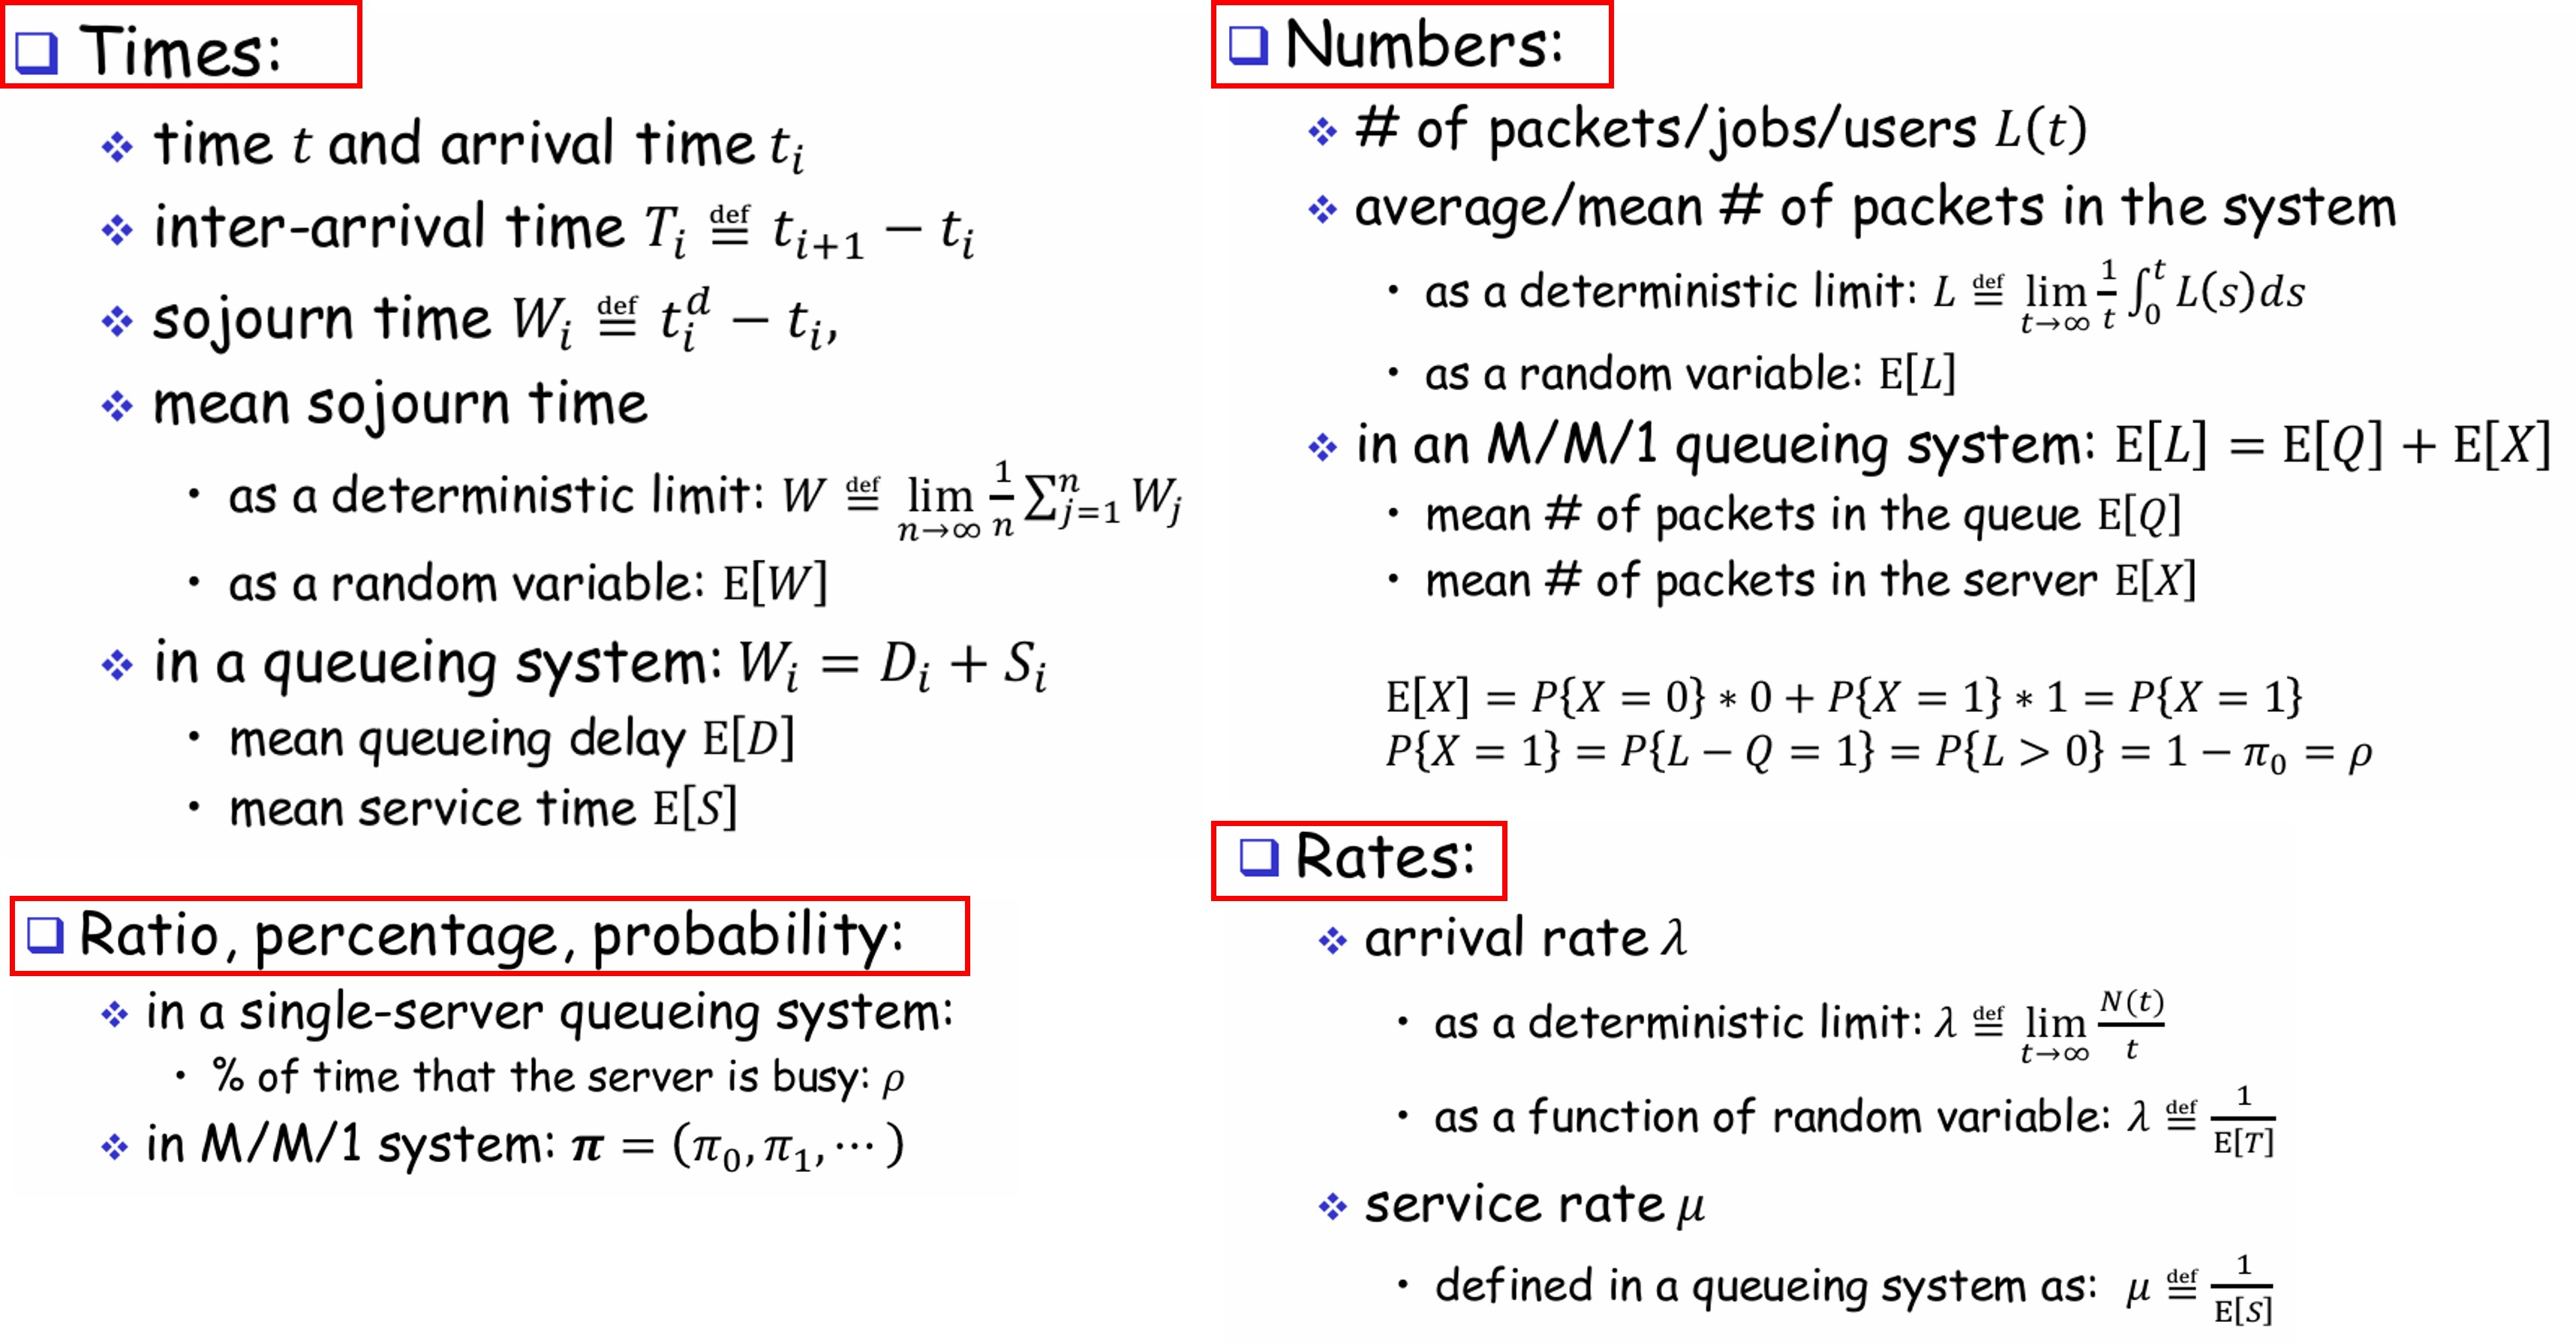
\includegraphics[width=1\linewidth]{notations}}
\null

\subsection{Effective Bandwidth}
\begin{itemize}
    \item Physical link capacity: theoretical hardware processing limit (E.g. 10Mbps cable)
    \item \textbf{Effective bandwidth}: actual throughput achievable, given service quality constraints. E.g. for $\mu$ capacity of M/M/1 link:
    \item (utilization constraint of $\rho \le \hat{\rho}$ , low delay (delay bounded by  $D \le \hat{D}$, where $E[D] = \frac{\rho}{\lambda - \mu} $, low loss etc) .
\end{itemize}

\subsection{Statistical Multiplexing vs Time Division Multiplexing}
\begin{itemize}
	\item \textbf{Time Division Multiplexing (TDM)}: Each of k users given fixed fraction of link capacity $\mu/k$, regardless of idleness (wasted capacity).
    \item With $k$ streams, $\rho = \frac{\lambda}{\mu} = \frac{\lambda/k}{\mu/k} = \rho$ (same server utilization), but avg. sojourn time ($E[W]$) increased by $k$ times under TDM. Queue length ($E[Q]$) and total users ($E[L]$) also $k$ times larger
    \item \textbf{Statistical Multiplexing}: Multiple traffic streams share the common link dynamically, each flow sends when has data, link schedules packets one by one from queue, bandwidth allocated statistically (random arrivals), not deterministically. (e.g. M/M/1 FIFO queue model)
    \item Statistical better than TDM. (same utilization, average less delay, shorter queue).
\end{itemize}

\subsection{Variants of Queueing Models}
\begin{itemize}
    \item Multiple servers: M/M/2, Limited queue size: M/M/1/K
    \item Different service: M/M/1/LIFO, General distributions: M/G/1, G/M/1, G/G/1
\end{itemize}

\subsection{\underline{Burke’s Theorem}}
\begin{itemize}
	\item For \textbf{M/M/1 queue} in steady state with arrival rate $\lambda$ and service rate $\mu > \lambda$
    \item \textbf{Departure} process of form Poisson process of rate ($\lambda$)
    \item \textbf{Independence}: System size at time $t$ independent of past departure times
    \item Implication is that output of one M/M/1 queue can be treated as Poisson input for the next queue, simplifying analysis of multi-hop queueing systems.
\end{itemize}

\subsection{Tandem Queues}
\begin{itemize}
	\item \textbf{Tandem Queue}: System where jobs pass through multiple servers in sequence, one after another. Each server $i$ modelled as an M/M/1 queue with own service rate, and utilization of server $i$: $\rho_i = \lambda / \mu_i$
    \item Joint probability of queue lengths (independent):
    \[
        P(L_1=j, L_2=k) = (1-\rho_1)\rho_1^j (1-\rho_2)\rho_2^k
    \]
\end{itemize}

\subsection{\underline{Jackson Network of Queues}}

\begin{itemize}
	\item Firstly, a \textbf{Acyclic Network with Probabilistic Routing} is where jobs arrive at a network node, and choose next node randomly. Poisson property preserved, departures remain independent Poisson processes (Poisson splitting)
    \item \textbf{Jackson Network}: Network of queues (e.g. M/M/1) with probabilistic routing  between servers $P_{ij}$, and can be acyclic or have feedback (cyclic).
\end{itemize}
\centerline{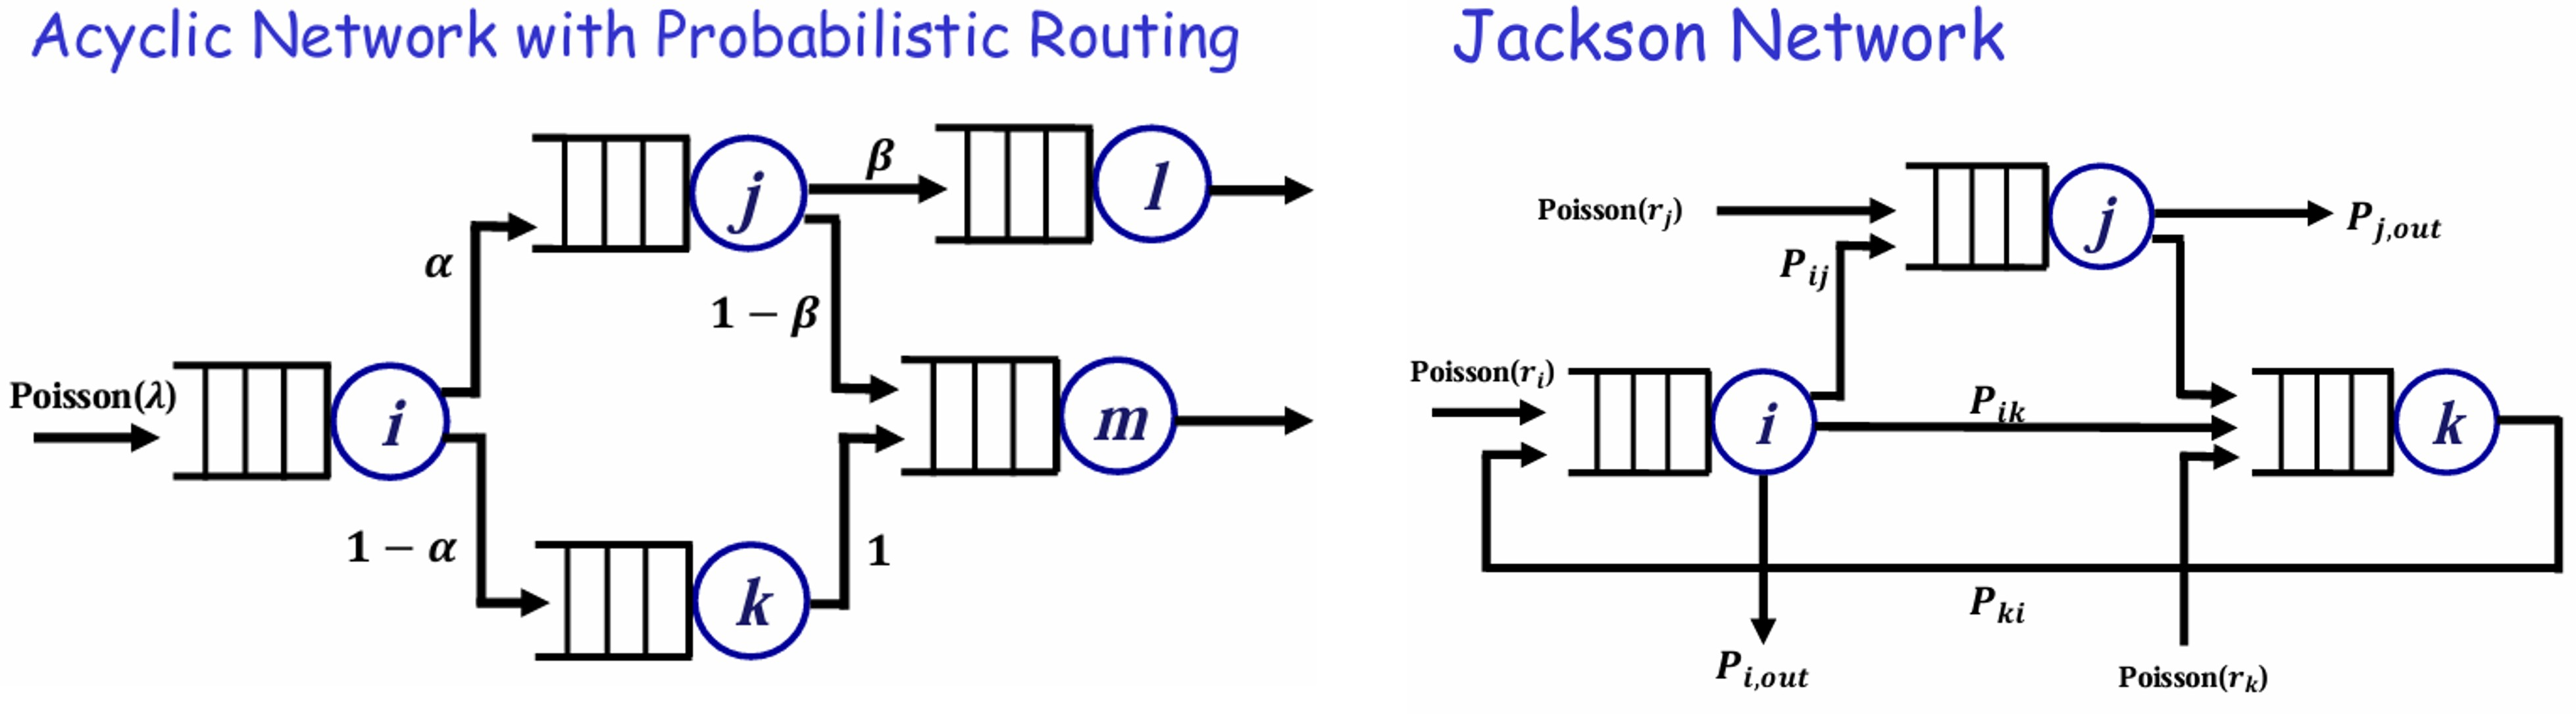
\includegraphics[width=1\linewidth]{jackson}}	    
\begin{itemize}
	\item \textbf{Solve Jackson Network}, Burke's theorem merge \& split of Poisson still apply. 
	\item \textbf{Two-step procedure}: determine utilization $\rho_i$ for each server, and product form solution.
    \item \underline{Effective arrival rate}: $\lambda_i$ at server $i$: $\lambda_i = r_i + \sum_{j=1}^n \lambda_j P_{ji} $ ($r$ is outside arrival)
    \item In matrix form: $\lambda = r + \lambda P \quad \Rightarrow \quad \lambda = r (I-P)^{-1}$
    \item Product form solution: $P(L_1=l_1, \dots, L_n=l_n) = \prod_{i=1}^n (1-\rho_i)\rho_i^{l_i}$
\end{itemize}

\subsection{Example Jackson Network: Web Server}
\centerline{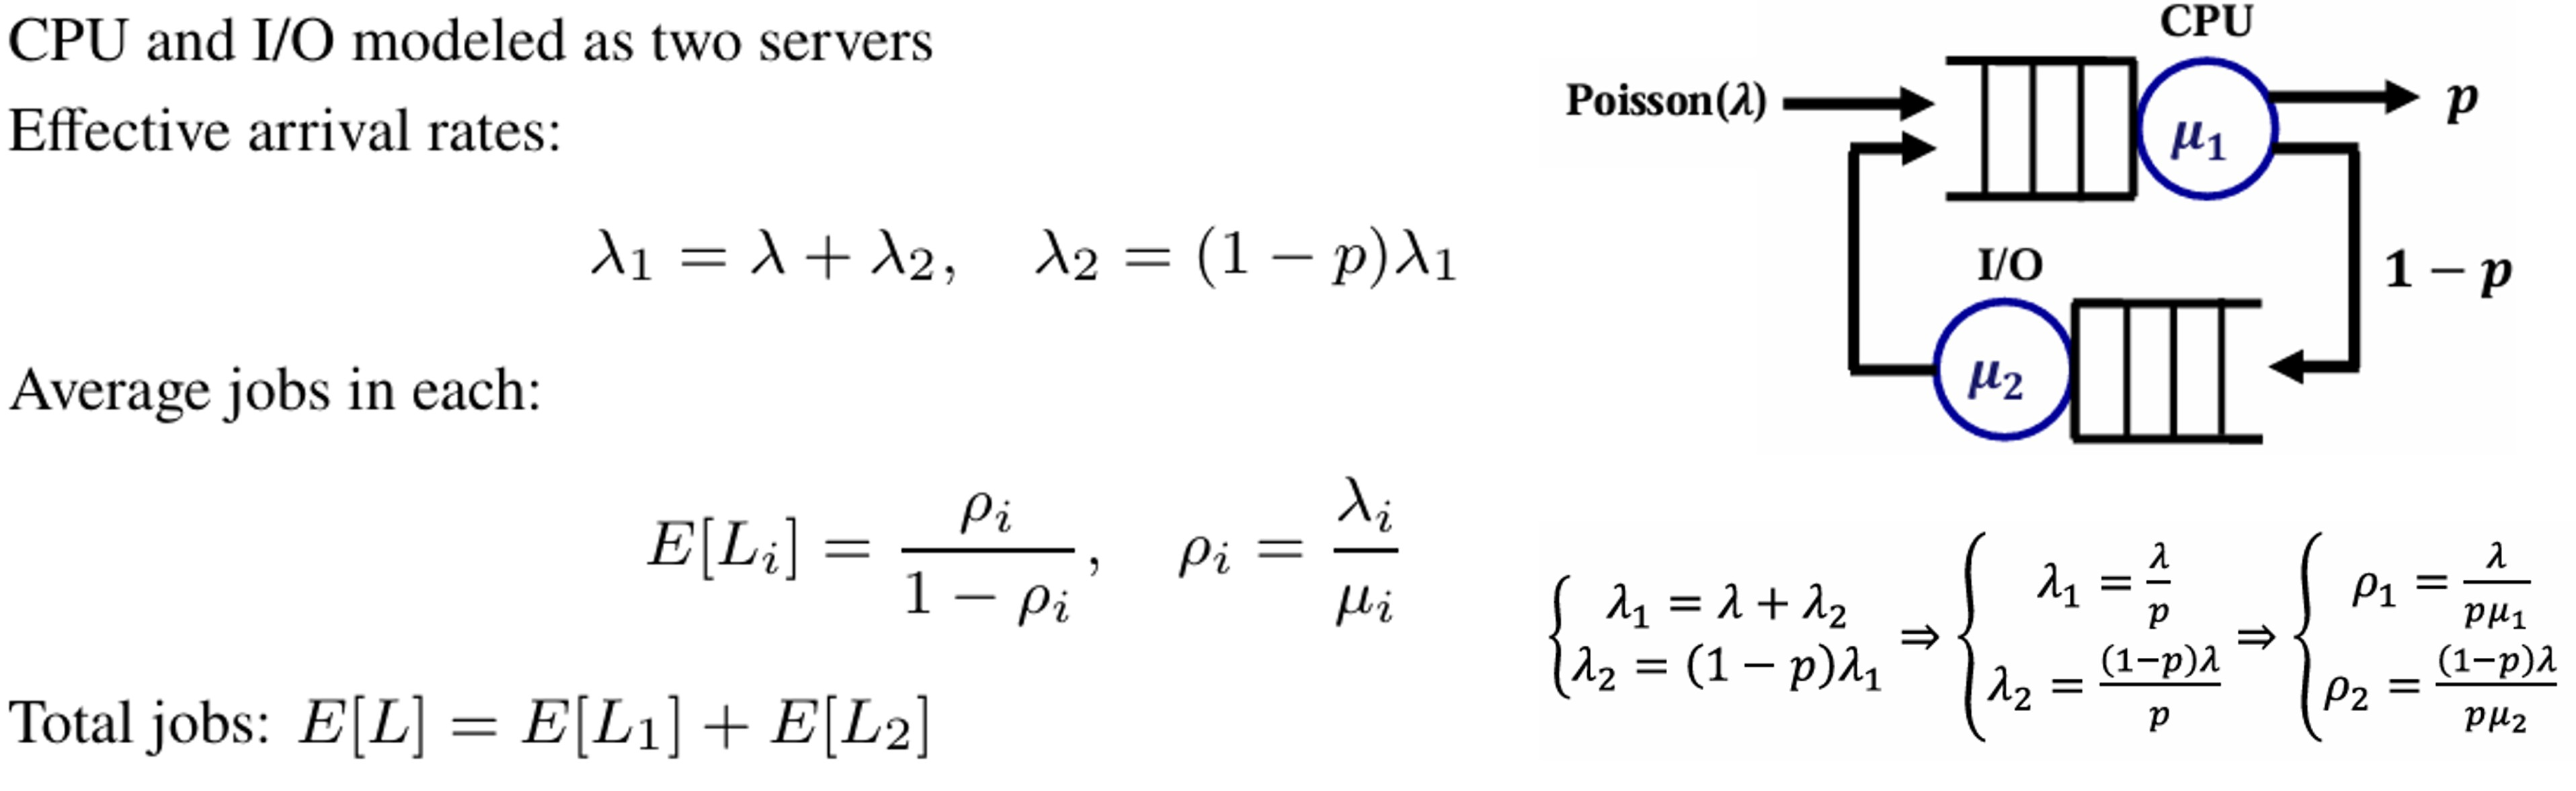
\includegraphics[width=1\linewidth]{webServer}}	    





















\end{multicols*}
\end{document}
